\apendice{Documentación de usuario}

\section{Introducción}
Puede ser que el usuario tenga dudas sobre el producto entregado o el manejo de este. En este anexo se ofrecerá toda la información que el usuario puede requerir para hacer un uso adecuado del producto entregado.

\section{Requisitos de usuarios}
El único requisito para que el usuario pueda ejecutar el videojuego es tener un ordenador con un sistema operativo Windows o Linux.

La otra preocupación del usuario puede ser que su ordenador no sea capaz de correr el juego debido a que es demasiado exigente. Es cierto que esto puede ocurrir con algunos juegos, pero suelen ser juegos de proporciones titánicas, con muchos eventos ocurriendo simultáneamente y con gráficos mucho más sofisticados que los de este juego.\\
A pesar de que se tiene la firme creencia firme de que puede ejecutar en prácticamente cualquier ordenador se van a listar las especificaciones de los dos ordenadores sobre los que se ha ejecutado el juego y comprobado su correcto funcionamiento.

\subsection{Predator PH315-51}
\begin{itemize}
\item
Procesador Intel Core i7-8750H (6 núcleos, 9 MB Caché, 2.2 GHz hasta 4.1 GHz)
\item
Memoria RAM de 16 GB DDR4 (alcanzando un pico de 141 MB cuando se ejecuta)
\item
Disco HDD de 1 TB
\item
Disco SSD de 128 GB
\item
Tarjeta gráfica Nvidia GeForce GTX 1060
\item
Sistema operativo Windows 10 Home
\end{itemize}

\subsection{Ordenador de ofimática}
\begin{itemize}
\item
Procesador Intel Core i3-6006U (2 núcleos, 3 MB Caché, 2 GHz)
\item
Memoria RAM de 4 GB DDR4
\item
Disco SSD de 200 GB
\item
Tarjeta gráfica Intel HD Graphics 520 (integrada)
\item
Sistema operativo Windows 10 Home
\end{itemize}

En ambos ordenadores el videojuego funciona sin ralentizaciones ni caídas de frames. Es cierto, aun así, que el ordenador de ofimática tarda un par de segundos más en cambiar entre escenas más que el otro ordenador (mucho más potente).

\subsection{Linux}
Para sistemas operativos Linux se ha ejecutado el juego en un ordenador con las siguientes especificaciones:
\begin{itemize}
\item
Procesador Intel(R) Core(TM) i3-5005U CPU (4 núcleos, 3 MB Caché, 2 GHz)
\item
Memoria 8 GB (usando algo menos de 116 MB cuando se ejecuta)
\item
Tarjeta gráfica Intel HD Graphics 5500 (integrada)
\item
Sistema operativo Ubuntu 20.04.1
\end{itemize}

\subsection{Requisitos mínimos}
Partiendo de las pruebas hechas se puede generar un listado de recursos mínimos que consumirá la ejecución del videojuego:
\begin{itemize}
\item
130 MB de disco duro los ficheros que contienen el juego (en la versión de Linux que es la que más ocupa)
\item
150 MB de RAM
\item
El procesador de gama más baja con el que se ha confirmado el correcto funcionamiento ha sido el procesador Intel Core i3-6006U (2 núcleos, 3 MB Caché, 2 GHz)
\item
La tarjeta gráfica de gama más baja con la que se ha confirmado el correcto funcionamiento ha sido la tarjeta gráfica Intel HD Graphics 5500
\end{itemize}

\section{Instalación}
El usuario no tendrá que instalar nada para poder iniciar el videojuego. Bastará con que se descargue el contenido del repositorio de GitHub asociado al proyecto (\url{https://github.com/Kencho/mri1001-tfg}).

Una vez descargado el repositorio, dentro de la carpeta executables, habrá tres ficheros comprimidos (game\_Windows.zip, game\_Linux.tar.gz y game\_WebGL.zip) que contendrán la estructura de ficheros del videojuego y el ejecutable que permitirá iniciarlo.

El usuario solo tendrá que descomprimir el fichero asociado a su sistema operativo o el fichero de WebGL si no se quiere estar atado a ningún sistema operativo. Después tendrá que entrar en la carpeta generada y ejecutar el fichero .exe. Esto iniciará la ejecución del videojuego.

\subsection{Instalación WebGL}
Sin embargo, es importante mencionar que para la versión de WebGL es necesario que el buscador con el que lo abres soporte WebGL. Esto se puede comprobar accediendo al siguiente enlace: \url{https://get.webgl.org/}.\\ 
Al entrar en esta página hay dos opciones: visualizar un cubo rotando o no visualizarlo. Si se visualiza significa que el navegador soporta WebGL.\\
Lo más probable es que cualquier navegador moderno popular que utilices soporten WebGL. Aun así, se ha comprobado empíricamente que los siguientes navegadores soportan WebGL:
\begin{itemize}
\item
Google Chrome
\item
Mozilla Firefox
\item
Microsoft Edge
\item
Internet Explore
\item
Opera
\end{itemize}

En caso de que no se vea el cubo rotando, lo más probable es que con actualizar los Drivers de la tarjeta gráfica se solucione el problema.

\clearpage
\begin{figure}[h]
\centering
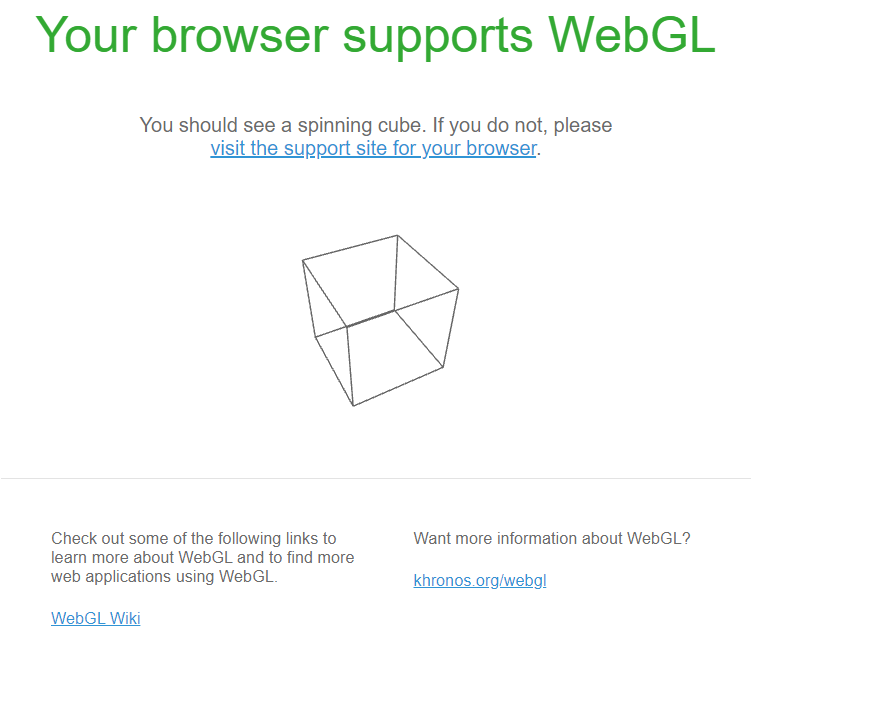
\includegraphics[scale=0.65]{Anexos/Anexo_E/Cubo_WebGL}
\caption{Cubo que rota si el navegador soporta WebGL}
\end{figure}

Aunque el navegador soporte WebGL, es muy probable que al ejecutar el fichero .html que inicia la ejecución en WebGL salte un error.

\begin{figure}[h]
\centering
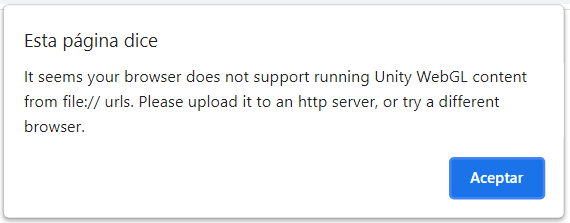
\includegraphics[scale=0.65]{Anexos/Anexo_E/Error_WebGL}
\caption{Error de la versión del ejecutable de WebGL}
\end{figure}

Este error no es realmente un error, sino una restricción de permisos. Los navegadores suelen tener una opción de seguridad que impide a las páginas acceder a recursos file://. Sin esta restricción se podría acceder a los ficheros del equipo, lo cual es una gran riesgo.\\
Para poder ejecutar el juego en WebGL sin hacer uso de un servidor web es necesario desactivar esta opción. Esta opción se puede desactivar siguiendo los pasos de explicados en el siguiente enlace: \url{https://bit.ly/3iEMWAj}.\\
Esta versión del ejecutable no es recomendable que un usuario que solo quiera disfrutar del videojuego la use. Ha sido añadida como opción para el desarrollo, esperando que se aloje en un servidor web.

\section{Manual del usuario}
Bienvenido, \textit{\textbf{JUGADOR}}, a nuestro nuevo videojuego. Ha habido un \textcolor{endeavour}{cataclismo intergaláctico} y los \textcolor{azulWorker}{ciber trabajadores espaciales} se han extraviado de camino a sus oficinas.


¿Serán capaces de volver los \textcolor{azulWorker}{ciber trabajadores} a la oficina para que puedan generar beneficios a la empresa antes de que se vuelvan un lastre y los despidan?

Se trata de un Plataformas 2D dónde podrá controlar a los \textcolor{azulWorker}{ciber trabajadores} y hacer uso de todas las herramientas de modificación del espacio y el tiempo que les provee su generoso jefe para recorrer el \textcolor{endeavour}{espacio multidimensional}.\\
Pero cuidado, muchos son los peligros que les aguardan y extraño el camino que ahora lleva hasta las oficinas.

\subsection{Controles}
Al iniciar el juego se encontrará con el menú principal. Desde él podrá seleccionar que \textcolor{azulWorker}{trabajador} desea ayudar a llegar a la oficina (como el 30 veces consecutivas empleado del mes, PruebaPlayerScene, o el irreemplazable conserje PruebaMovingObstacleScene).

¡Seleccione a que \textcolor{azulWorker}{trabajador} desea ayudar y tome posesión de su cuerpo para asegurarse de que no le despidan!

Pero igual no esta muy ducho en el arte de poseer \textcolor{azulWorker}{trabajadores}, o incluso de navegar por los abstractos \textit{''Menús del juego''}, que por supuesto no existen en otro \textcolor{endeavour}{plano astral} completamente distinto al de los \textcolor{azulWorker}{trabajadores}.

No pasa nada, \textit{\textbf{JUGADOR}}, vallamos paso a paso.

\subsubsection{Controles del menú principal}
Para navegar por los menús del juego solo tendrá que tener claro que botón está seleccionado ahora mismo. Eso lo sabrá porque, a diferencia del resto de botones, de color \textcolor{fucsia}{rosa fucsia}, el botón seleccionado será de color \textcolor{flirk}{rosa flirt}.

Ahora que usted,  \textit{\textbf{JUGADOR}}, sabe en qué botón se encuentra solo necesita saber que acciones puede realizar desde él.
\begin{itemize}
\item
Podrá ir al rescate accediendo al nivel jugable pulsando el botón ''X'' de su mando (entendemos está usando una mando de Play Station) o la tecla ''ENTER'' de su teclado. En cuanto lo haga viajará al \textcolor{endeavour}{esperpéntico mundo} en el que el \textcolor{azulWorker}{trabajador} espera a ser devuelto a su oficina.
\item
Si le cae mal ese \textcolor{azulWorker}{trabajador} en particular y desea salvar a otro, podrá desplazarse al botón en el que se encuentra su \textcolor{azulWorker}{\textbf{trabajador favorito}} y acudir en su rescate.\\
De un botón se podrá viajar a otro de la siguiente manera:
\begin{itemize}
\item
Si desea desplazarse al botón que se encuentra sobre el botón seleccionado empuje el Stick izquierdo del mando hacia arriba o pulse la flecha que apunta hacia arriba del teclado.
\item
Si, en cambio, desea desplazarse al botón que se encuentra bajo el botón seleccionado empuje el Stick izquierdo del mando hacia abajo o pulse la flecha que apunta hacia abajo del teclado.
\item
Si el desplazamiento vertical entre botones lo tiene dominado pruebe a  desplazarse al botón que se encuentra a la derecha del botón seleccionado. Empuje el Stick izquierdo del mando hacia la derecha o pulse la flecha que apunta hacia la derecha del teclado.
\item
Quiza le parezca, \textit{\textbf{JUGADOR}}, una decisión de diseño arriesgada, pero si desea desplazarse al botón que se encuentra a la izquierda del botón seleccionado empuje el Stick izquierdo del mando hacia la izquierda o pulse la flecha que apunta hacia la izquierda del teclado.
\end{itemize}
\item
Es posible que la misteriosa música que ha invadido el universo (o todo sonido en general) le resulte molesta. Viaje al menú de opciones y cambie asígnele el valor que desee al volumen. Puede acceder al menú de opciones seleccionando el botón ''Options''.
\item
Si está cansado de los \textcolor{azulWorker}{trabajadores} se aprovechen de tu buena fe para llegar al trabajo sin dar palo al agua y desea abandonarles a su suerte, no pasa nada. Cierre el juego pulsando el botón de ''Exit'' y tómese unas merecidas vacaciones que se descontarán de su sueldo.\\
Pero ¡cuidado!, es posible que los \textcolor{azulWorker}{trabajadores} sigan en su sitio a la espera de ser rescatados cuando vuelva a abrir el juego.
\end{itemize}

\begin{figure}[h]
\centering
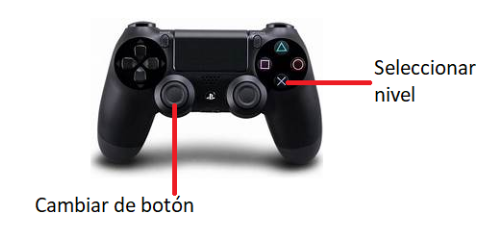
\includegraphics[scale=0.65]{Anexos/Anexo_E/Mando_menus}
\caption{Controles de mando del menú}
\end{figure}

\begin{figure}[h]
\centering
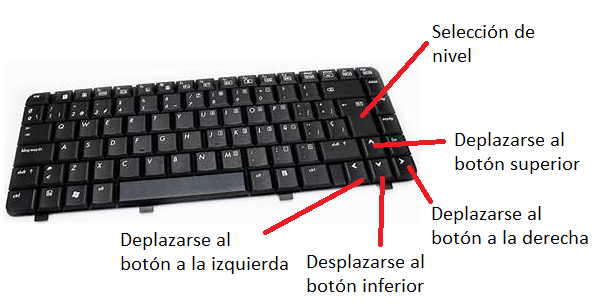
\includegraphics[scale=0.65]{Anexos/Anexo_E/Teclado_menus}
\caption{Controles de teclado del menú}
\end{figure}

\subsubsection{Menú de pausa}
Se encuentra, \textit{\textbf{JUGADOR}}, en el menú de pausa. Desde este menú podrá modificar el volumen general situándose sobre la barra de desplazamiento de ''General Volume'' (de la misma forma que se hace con los botones del menú principal).\\
Empujando el Stick izquierdo del mando hacia la derecha o pulsando la flecha que apunta hacia la derecha del teclado se aumentará el volumen general.\\
Empujando el Stick izquierdo del mando hacia la izquierda o pulsando la flecha que apunta hacia la izquierda del teclado se reducirá el volumen general.

Si solo se desea cambiar el volumen de la música deberá hacer lo mismo que para el volumen general pero seleccionando la barra de desplazamiento de ''Music Volume'' en vez de la de ''General Volume''.

\subsubsection{Controles de nivel jugable}
Ahora que domina los menús seleccione el \textcolor{azulWorker}{trabajador} al que desea salvar. Se encuentra ahora, \textit{\textbf{JUGADOR}}, en un \textcolor{endeavour}{mundo desconocido}, para colmo, manejando un cuerpo que no es el suyo. Ya que puede ser la primera vez que se encuentra en una situación tan comprometida como esta. No se preocupe, se le dará una ligera explicación de como maniobrar un cuerpo ajeno.
\begin{itemize}
\item
Para moverse a la izquierda empuje el Stick izquierdo del mando hacia la izquierda o pulse la flecha que apunta hacia la izquierda del teclado.
\item
Para moverse a la derecha empuje el Stick izquierdo del mando hacia la derecha o pulse la flecha que apunta hacia la derecha del teclado.
\item
El \textcolor{azulWorker}{trabajador} tiene la capacidad de saltar. Ordénele saltar pulsando el botón ''X'' del mando o la tecla ''Espacio'' del teclado.
\end{itemize}

Por sobrecogedora que resulte la capacidad de saltar del \textcolor{azulWorker}{trabajador} no es su as bajo la manga. Cuenta con dos mecánicas más:
\begin{itemize}
\item
La capacidad de realizar un acelerón en la dirección en la que está mirando. Podrá realizar esta acción pulsando el botón ''O'' del mando o la tecla ''S'' del teclado.
\item
Podrás forzar a tu \textcolor{azulWorker}{trabajador}, en contra de su voluntad, a reducir la velocidad a la que pasa el tiempo pulsando el botón ''R1'' del mando o la tecla ''D'' del teclado. Es recomendable que recuerde que el jugar con el tiempo tiene sus límites y cabo de unos pocos segundos la velocidad a la que pasa el tiempo volverá a su curso natural.
\end{itemize}


Es entendible que poseer un cuerpo que no le pertenece puede resultar agotador. Pulse el botón ''R2'' del mando o la tecla ''ESC'' del teclado para abrir el menú de pausa. Mientras el menú de pausa este activo, el tiempo se detendrá ofreciéndole un descanso hasta que cierre el menú de pausa (con los mismos controles). Puede ir a prepararse una leche con Nesquik con la tranquilidad de que nada atentará contra la vida del \textcolor{azulWorker}{trabajador}.

Desde el menú de pausa podrá modificar el volumen de las misma forma que desde el menú de opciones.

\begin{figure}[h]
\centering
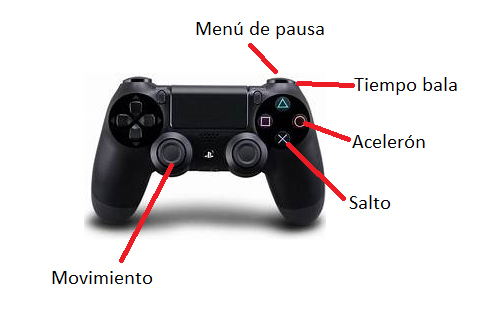
\includegraphics[scale=0.65]{Anexos/Anexo_E/Mando_juego}
\caption{Controles de mando de los niveles jugables}
\end{figure}

\begin{figure}[h]
\centering
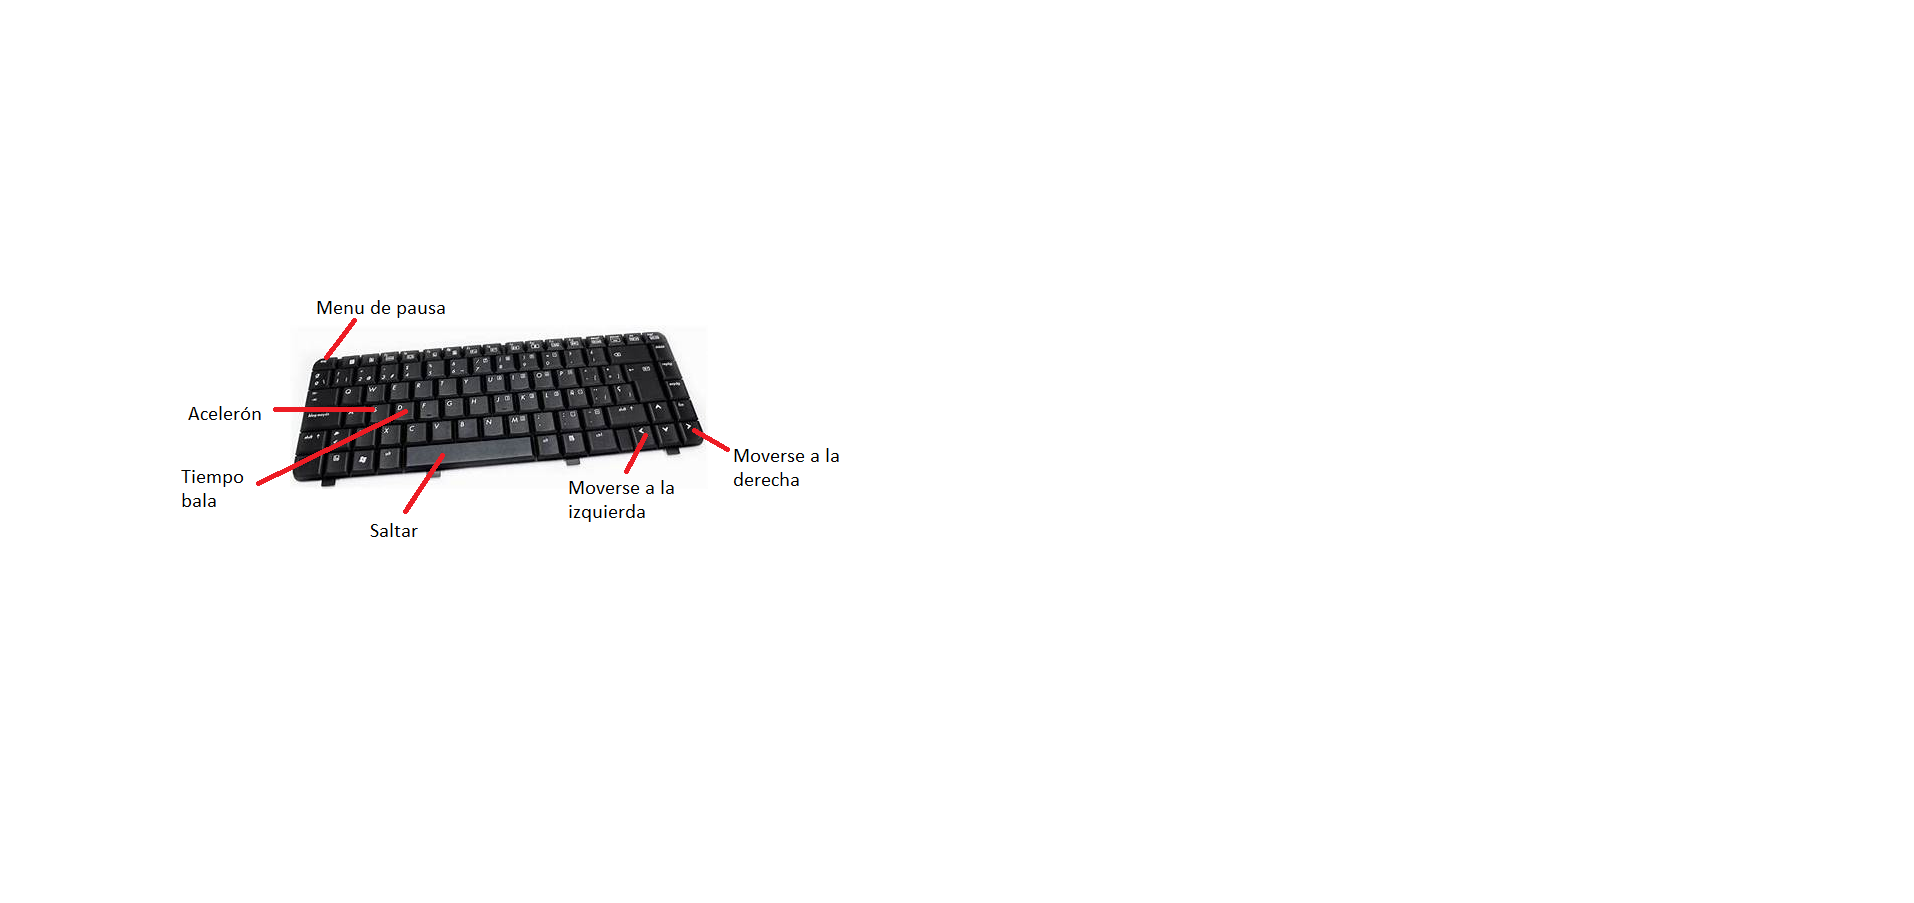
\includegraphics[scale=0.65]{Anexos/Anexo_E/Teclado_juego}
\caption{Controles de teclado de los niveles jugables}
\end{figure}